\documentclass[12pt,b5paper]{ltjsarticle}

% 余白
%\usepackage[margin=15truemm, top=5truemm, bottom=5truemm]{geometry}
%\usepackage[margin=10truemm,left=15truemm]{geometry}
\usepackage[margin=10truemm]{geometry}

% AMS math パッケージ
\usepackage{amsmath,amssymb}

%\pagestyle{headings}
\pagestyle{empty}

\renewcommand{\theenumi}{(\arabic{enumi})}

\usepackage{graphicx}

%\usepackage{tikz}
%\usetikzlibrary {arrows.meta}
%\usepackage{wrapfig}
%\usepackage{bm}

% ルビを振る
%\usepackage{luatexja-ruby}	% required for `\ruby'

%% 核Ker 像Im Hom を定義
%\newcommand{\Img}{\mathop{\mathrm{Im}}\nolimits}
%\newcommand{\Ker}{\mathop{\mathrm{Ker}}\nolimits}
%\newcommand{\Hom}{\mathop{\mathrm{Hom}}\nolimits}

%\DeclareMathOperator{\Rot}{rot}
%\DeclareMathOperator{\Div}{div}
%\DeclareMathOperator{\Grad}{grad}
%\DeclareMathOperator{\arcsinh}{arcsinh}
%\DeclareMathOperator{\arccosh}{arccosh}
%\DeclareMathOperator{\arctanh}{arctanh}

% URL出力
\usepackage{url}

% ソースコード出力
%\usepackage{listings}

%\usepackage{listings}
%
%\lstset{
%%プログラム言語(複数の言語に対応,C,C++も可)
%  language = Python,
%%  language = Lisp,
%%  language = C,
%  %背景色と透過度
%  %backgroundcolor={\color[gray]{.90}},
%  %枠外に行った時の自動改行
%  breaklines = true,
%  %自動改行後のインデント量(デフォルトでは20[pt])
%  breakindent = 10pt,
%  %標準の書体
%%  basicstyle = \ttfamily\scriptsize,
%  basicstyle = \ttfamily,
%  %コメントの書体
%%  commentstyle = {\itshape \color[cmyk]{1,0.4,1,0}},
%  %関数名等の色の設定
%  classoffset = 0,
%  %キーワード(int, ifなど)の書体
%%  keywordstyle = {\bfseries \color[cmyk]{0,1,0,0}},
%  %表示する文字の書体
%  %stringstyle = {\ttfamily \color[rgb]{0,0,1}},
%  %枠 "t"は上に線を記載, "T"は上に二重線を記載
%  %他オプション:leftline,topline,bottomline,lines,single,shadowbox
%  frame = TBrl,
%  %frameまでの間隔(行番号とプログラムの間)
%  framesep = 5pt,
%  %行番号の位置
%  numbers = left,
%  %行番号の間隔
%  stepnumber = 1,
%  %行番号の書体
%%  numberstyle = \tiny,
%  %タブの大きさ
%  tabsize = 4,
%  %キャプションの場所("tb"ならば上下両方に記載)
%  captionpos = t
%}


%\usepackage{cancel}
%\usepackage{bussproofs}
%\usepackage{proof}



% 出力用フォント
%\usepackage[ipaex]{luatexja-preset}% IPAexフォントしたい
%\renewcommand{\kanjifamilydefault}{\gtdefault}% 既定をゴシック体に



\begin{document}

\hrulefill

$x^{2}\cos{\frac{1}{x}}$の$x=0$における微分可能性

\dotfill


$f(x)=x^{2}\cos{\frac{1}{x}}$
とし、
$x=0$における微分係数$f^{\prime}(0)$を求める。

微分係数$f~{\prime}(0)$は
次のような極限で定義される。
\begin{equation}\label{def:diff}
 f^{\prime}(0)
  =
  \lim_{\Delta x \to 0}\frac{f(0+\Delta x)-f(0)}{\Delta x}
\end{equation}


まず、$f(0)$の値を求める。

$x\in\mathbb{R}\backslash \{0\}$において
$-1 \leq \cos{\frac{1}{x}} \leq 1$であるので、
$-x^{2} \leq f(x) \leq x^{2}$である。
つまり、$y=f(x)$ は
$y=-x^{2}$と$y=x^{2}$
の間にグラフが描かれる。 

% グラフ
\begin{center}
 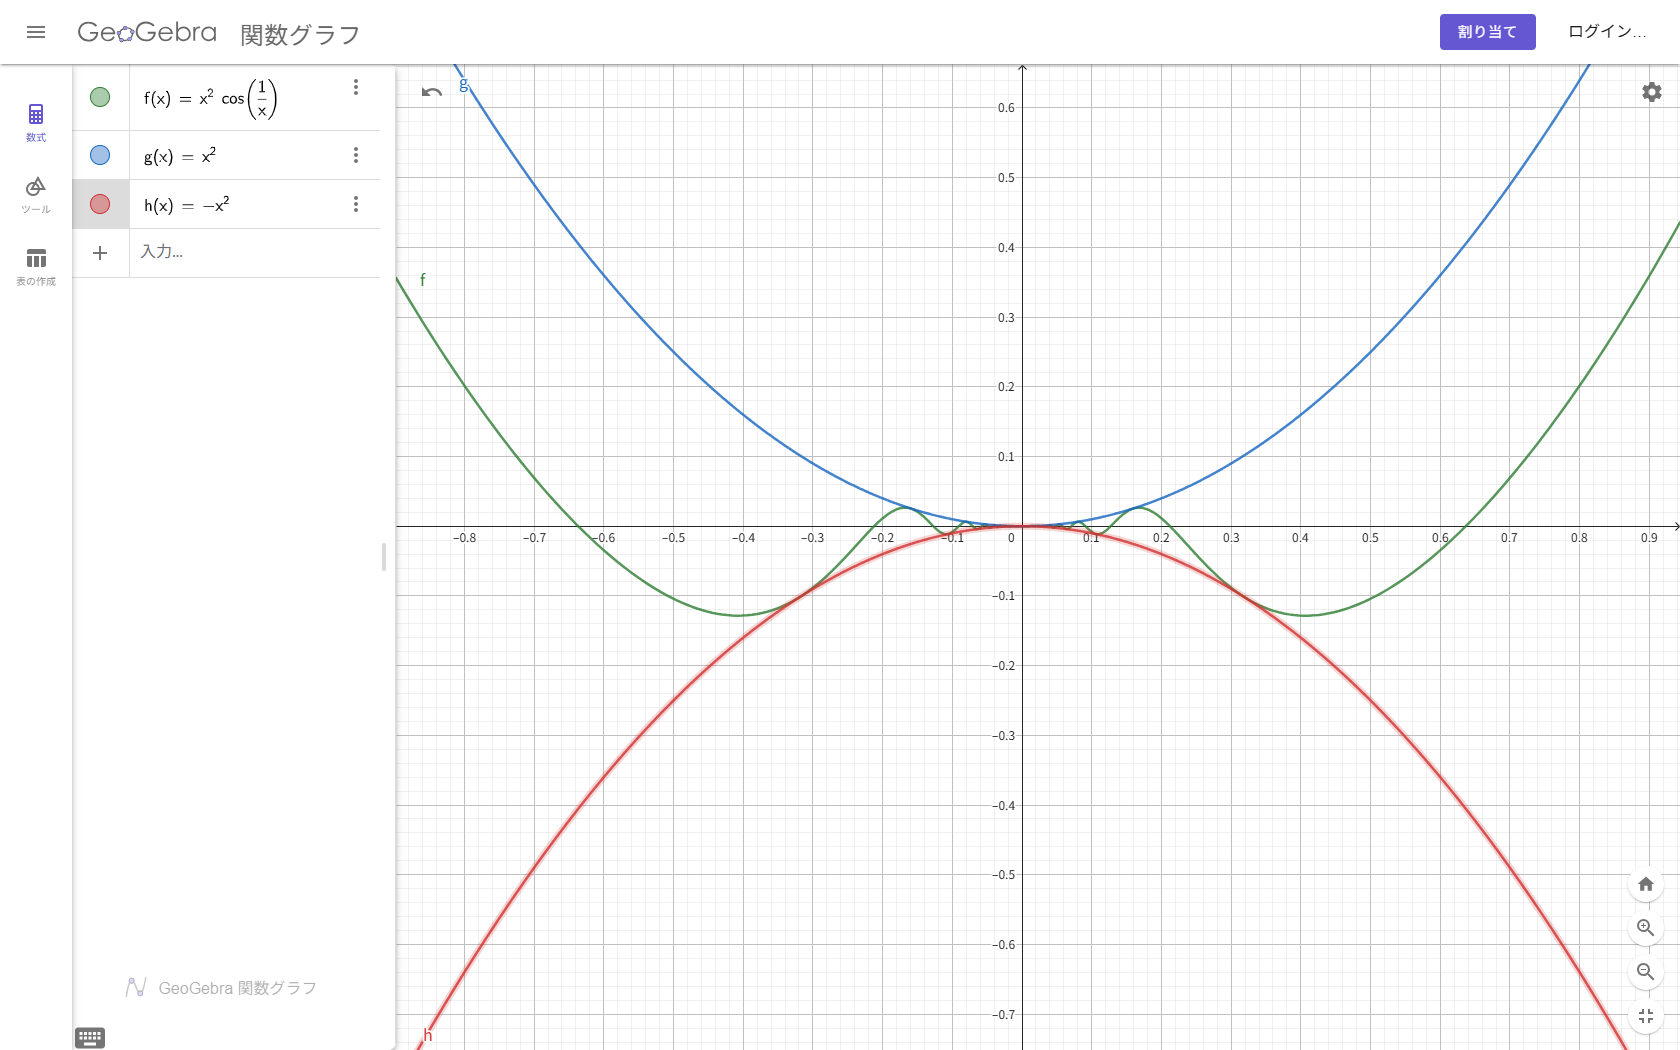
\includegraphics[scale=0.34]{graph_x2.png}
\end{center}



$x=0$としてみれば、
$0 \leq f(0) \leq 0$となるので、
$f(0)=0$と定義すると都合が良い。

そこで、
$f(0)=0$として
\eqref{def:diff}
に当てはめると次のようになる。
\begin{align}
  \lim_{\Delta x \to 0}\frac{f(0+\Delta x)-f(0)}{\Delta x}
  & =
  \lim_{\Delta x \to 0}\frac{f(\Delta x)}{\Delta x}\\
  & =
  \lim_{\Delta x \to 0}
  \Delta x \cos{\frac{1}{\Delta x}}
 =0
\end{align}

つまり、$f^{\prime}(0)=0$である。

$f^{\prime}(0)$
の値が存在するので、
$f(0)=0$とするなら
$x=0$において微分可能である。

\begin{equation}
 f(x)=
 \begin{cases}
  0 & (x=0)\\
  x^{2}\cos{\frac{1}{x}} & (\text{otherwise})
 \end{cases}
\qquad
\Longrightarrow
\qquad
f^{\prime}(0)=0
\end{equation}

\hrulefill
\dotfill
\hrulefill
\dotfill
\hrulefill

$x^{2}\cos{\frac{1}{x}}$
の導関数を公式を用いて求める。

\begin{align}
 \left(x^{2}\cos{\frac{1}{x}}\right)^{\prime}
  & =
  (x^{2})^{\prime}\cos{\frac{1}{x}}
  +
  x^{2} \left( \cos{\frac{1}{x}} \right)^{\prime}\\
  & =
  2x\cos{\frac{1}{x}}
  +
  x^{2} \left(- \sin{\frac{1}{x}} \right) \left(\frac{1}{x}\right)^{\prime}\\
  & =
  2x\cos{\frac{1}{x}}
  +
  x^{2} \left(- \sin{\frac{1}{x}} \right) \left(-\frac{1}{x^{2}}\right)\\
  & =
  2x\cos{\frac{1}{x}}
  + \sin{\frac{1}{x}}
\end{align}

\end{document}
